
% \begin{document}

There are several existing approaches about Visualizing Data 2D, 3D, Flash, Flex, Mobile, among others \cite{SeveralSurveys}, \cite{Dadzie2011}, \cite{IJST38378}. This works are relevant to our work, but our main goal are more focused to LOD CLoud Diagram, in order to do a new Visualization of this Diagram that are updated and allow make-filters.

\subsection{lod-cloud.net: The Linking Open Data cloud diagram}
This work is our main motivation, because here we try to provide some improvements about the actual LOD Cloud Diagram \cite{lodcloud}.
The problems that we will try to provide some solution are: Up-to-dateness, because according the authors \cite{lodcloud}, \textbf{"This image shows datasets that have been published in Linked Data format, by contributors to the Linking Open Data community project and other individuals and organisations. It is based on metadata collected and curated by contributors to the Data Hub as well as on metadata extracted from a crawl of the Linked Data web conducted in April 2014."}.

Therefore, we can notice that this Graph is not updated automatically, because the last updated was: 2014-08-30, and of course, not allowing filters, because is an static image.


\subsection{VoID-graph}
VoID-graph \cite{Voidgraph} is a standalone web-tool that, given a VoID description, can visualize a diagram similar to the LOD cloud \cite{lodcloud}, is built using Open Web standards such as JavaScript, HTML5, CSS3 and SVG. Users can simply download the source-code and run the index.html file to utilize the tool from the webSite. Compared to other software, which requires the configuration of specific runtimes and the installation of a variety of dependencies, VoID-graph can more easily be hosted and installed on a variety of systems.

\subsection{LOD Cloud VoID Generator}
This work \cite{VoIdGenerator} is responsable by generate a VoID description of all datasets in the lodcloud group on the Data Hub.

This project is about generating a VoID description of all the datasets in the LOD Cloud diagram. It currently generates an RDF dump containing these descriptions, available online here:\footnote{\url{http://lod-cloud.net/data/void.ttl}}

The LOD Cloud diagram is a pictorial of datasets published in linked data format on the Web.
Metadata for these datasets is recorded in the Data Hub, an open directory of datasets. The lodcloud group contains metadata for all the datasets in the LOD Cloud diagram.
VoID is an RDF vocabulary for expressing metadata about such datasets in RDF format.
At some point, this project was intended to produce not just an RDF dump, but also RDF and HTML descriptions of each entity described in the dump. That effort stalled, and is removed from the current codebase, but can still be found in the feature-html branch.

Source-code for lod-cloud.net \cite{lodcloud}, can be found here:\footnote{ \url{https://github.com/lod-cloud/lod-cloud}}, the website of the Linked Open Data Cloud diagram \cite{lodcloud}.

\subsection{DataHub2Void}
There are an work \cite{Datahub2Void} that generates a VoID description of all datasets in the lodcloud group on the Data Hub.

\subsection{LOD for all}
This work \cite{lod4all} provides an LOD Cloud Diagram, that have some particularities, such as, when you keep you mouse pointer under an bubble, a kind of sub graph is showed. Allow make filters as well. Therefore this feature brings an easy way comparing with others that makes this work be relevant.
This work is licensed under a Creative Commons Attribution 3.0 Unported License. creative commons license. Copyright © 2014 FUJITSU LABORATORIES LTD.

Includes additional datasets beyond those that are officially part of the “lodcloud” group. Also include datasets that have been tagged with the “lod” tag (according to metadata collected from Datahub) and that follow the license criteria explained above.

Is interactive. You can filter datasets based on several criteria, zoom and pan around the diagram and select a dataset with a click to inspect its links to other datasets, or with a double-click to see the dataset details page.

\subsection{Towards a Dynamic Linked Data Observatory (DynLOD)}
The Dynamic Linked Data Observatory \cite{dynlod} is a framework to monitor Linked Data over an extended period of time. The core goal of our work is to collect frequent, continuous snapshots of a subset of the Web of Data that is interesting for further study and experimentation, with an aim to capture raw data about the dynamics of Linked Data. The resulting corpora will be made openly and continuously available to the Linked Data research community.

Until now, they provide weekly crawls and updated.

The newest crawl dumps should be available for download \footnote{\url{http://swse.deri.org/dyldo/data/}} roughly one day after they got crawled.

This work \cite{dynlod} proposes an way to monitoring Linked Open Data around the Web.
One possible problem is that data format, because we cannot found an specific format such as turtle, VoId Description or another one.

\subsection{Protovis} 
Protovis \cite{Protovis} was already been analysed before in \cite{SurveyLODDiagram1}, but as complement we can tell that is a graphical approach to visualizing the LOD Cloud diagram using free and open-source under the BSD License. It uses JavaScript and SVG for web-native visualizations and no plug-in required.
The Protovis team is now developing a new visualization library called D3.js \cite{d3js}, with improved support for animation and interaction.
There is no way filter and the graph is manually updated.

\subsection{Czech LOD Cloud}
Czech LOD (CzLOD) cloud diagram \cite{app24} show a set of interlinked LOD datasets that they have published in your research group trying to show the benefits of the Linked Data Visualization Model (LDVM) for LOD visualization.
The data are not automatic updated and we cannot found a way to make filters.

\subsection{lodlive} 
LODLive \cite{lodlive1} is an environment that generates an Graph based in some filter in some predefined dataSets like dbPedia.org and freebase.org, you also can input an URI.
This work allow make filters, but the result graph/Graph is not properly similar to LOD Cloud Diagram \cite{lodcloud}.
An suggestion maybe could be put a kind of automatically search for all datasets, could be direct in DataHub.io.

\subsection{rkbexplorer} 
The rkbexplorer \cite{rbkexplorer} presents a tool that provides an graphical environment. An good point is that according the literature \footnote{\url{http://lists.w3.org/Archives/Public/public-lod/2009Jan/0061.html}} that shows is  possible to generate a LOD Cloud Diagram using this tool and also allowing filters.

\subsection{Callimachus}
This work initiallly \cite{callimachus} is an tool for visualizing Linked Data, but still here because this tool can reproduce the LOD Cloud Diagram as well, but in his webSite \footnote{ \url{http://semanticweb.com/tag/callimachus-project}} is explained that is not a intention of this tool. Therefore, this is not a good way to adote this tool, unless we have only this way.

\subsection{Gephi: Semantic Web Crawling Visualization}
This approach \cite{WebCrawlVis} provide some examples and visualizations of semantic web crawls using Gephi \footnote{\url{http://gephi.github.io/}} as graph visualiser and LDSpider as semantic crawler, that allow filters, but not provide automatic update.
This work can be used as LOD Cloud Digram as well, because as lod-cloud.net use LDSpider to crawling the data.


\section{Criteria}
In order to provide a explanation about the criteria adopted in this work which allow to evaluate tools and approaches.

\paragraph{Data Updated Automatically:} The work needs to provide data that are automatically updated, in order to provide always an updated and reliable LOD Cloud Diagram.

%List of approaches that can help keep Data Updated Automatically:
%\begin{itemize}
%\item Ping the Semantic Web API  \footnote{\url{http://www.programmableweb.com/api/ping-semantic-web}}. %This work can be used to check if an Document is really updated.

%The API allows you to notify when you created/updated an RDF document on your web site. You can also %import the list of recently created/updated RDF documents.

%\item "AKSW Semantic Pingback" \footnote{\url{http://aksw.org/Projects/SemanticPingback.html}}.
%\end{itemize}

\paragraph{Allow filter:} In order to provide an way to make sub LOD CLoud diagrams about specific subjects, for example, an sub LOD Cloud about Librarians. 

\begin{table}[htbp]
\caption{Selected approaches and criteria }
\begin{tabular}{|l|c|c|c|}
\hline
 & \multicolumn{ 3}{c|}{\textbf{Criteria}} \\ \hline
\multicolumn{1}{|c|}{\textbf{Approach / Tool}} & \textbf{Updated} & \textbf{Allow Filter} & \textbf{Web} \\ \hline
lod-cloud.net  &  &  & x \\ \hline
LOD for all &  & x & x \\ \hline
DynLOD & x &  & x \\ \hline
Protovis &  &  & x \\ \hline
VoID &  &  & x \\ \hline
LODLive &  & x &  \\ \hline
rkbexplorer &  & x & x \\ \hline
Callimachus &  & x & x \\ \hline
Gephi\\Crawling Visualization &  & x &  \\ \hline
\end{tabular}
\label{Criteria}
\end{table}

\section{Linked Data Browsers}

Linked Data Browsers can be an way to visualise LOD-cloud diagrams, thus, the work by Dadzie 2011 \cite{Dadzie2011} shows key requirements and approaches, such as two tables represented by figures ~\ref{fig:crit1} and ~\ref{fig:crit2} that can represent some criteria comparing 15 tools to visualising Linked Data.

\begin{figure*}[tbp] 
  \centering
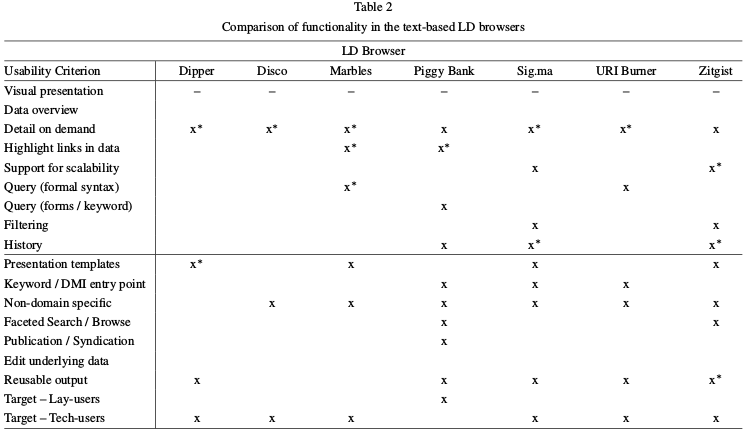
\includegraphics[width=\textwidth]{img/table2.png}
  \caption{Criteria about LD Browsers (1-2) \cite{Dadzie2011}}
  \label{fig:crit1}
\end{figure*}

\begin{figure*}[tbp] 
  \centering
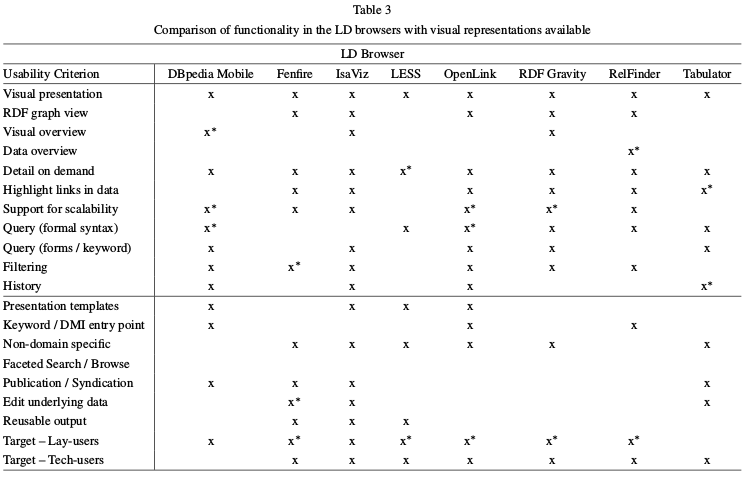
\includegraphics[width=\textwidth]{img/table3.png}
  \caption{Criteria about LD Browsers (2-2) \cite{Dadzie2011}}
  \label{fig:crit2}
\end{figure*}

\section{Steps to have you own LOD Cloud Diagram}

This steps are based in a tutorial provided by Luca Matteis \cite{Voidgraph} \footnote{\url{http://markmail.org/search/?q=+list\%3Aorg.w3.public-lod+lod+cloud+visualisation\#query:lod\%20cloud\%20visualisation+page:1+mid:xiwz5envzoeqbq3x+state:results}}.

\begin{enumerate}

\item Download all metadata about datasets already stored in http://datahub.io/. Use this script:

\footnote{\url{https://github.com/lod-cloud/datahub2void}}

to get a void.ttl file

\item Load void.ttl into your RDF storage server.

\item Make this query:

PREFIX rdfs:<\url{http://www.w3.org/2000/01/rdf-schema#}> \\
PREFIX foaf:<http://xmlns.com/foaf/0.1/> \\
PREFIX tag:<\url{http://www.holygoat.co.uk/owl/redwood/0.1/tags/}> \\
PREFIX owl:<\url{http://www.w3.org/2002/07/owl#}> \\
PREFIX xsd:<\url{http://www.w3.org/2001/XMLSchema#}> \\
PREFIX void:<\url{http://rdfs.org/ns/void#}> \\
PREFIX rdf:<\url{http://www.w3.org/1999/02/22-rdf-syntax-ns#}> \\
PREFIX skos:<\url{http://www.w3.org/2004/02/skos/core#}> \\
PREFIX dcterms:<\url{http://purl.org/dc/terms/}>

select * { ?s a void:Linkset. ?s void:linkPredicate skos:exactMatch. ?s void:objectsTarget ?otarget. ?s void:subjectsTarget ?starget. ?s void:triples ?triples. }

\item Export results of this query as N-triples.
\item Download \url{https://github.com/lmatteis/void-graph}. 
\item Open file index.html in your browser. Inside text area field, paste all n-triples you have already exported. 

\item That is all. You must have your own LOD - Cloud in a couple seconds. 
\end{enumerate}

\bibliographystyle{abbrv}
\bibliography{refs}


% \end{document}
